\label{sec:fake_leptons}
To estimate the expected fake lepton background yield in the signal region,
dedicated control regions are defined with requirements similar to the signal region but in such a way not to contain signal events.
To enhance the \nonprompt lepton component, events in these regions are required to
have a number of leptons that fail the tight selection, while passing the loose criteria.
The other selections are identical to maintain similarity with the signal region.

The fake lepton background yield in the signal region is extrapolated from these regions
according to the probability for loose lepton candidates to pass also the final selection criteria,
defined in Sections~\ref{sec:ele_selection} and \ref{sec:muo_selection} for electrons and muons respectively.
These probabilities, referred to as fake rates, are estimated independently as illustrated in the following section.

\subsubsection{Lepton fake rate measurement}
\label{sec:CRLFR}
The measurement of the lepton fake rate, which is the probability that a fake lepton that passes the loose selection also passes the tight criteria,
is carried out in a separate control region which is enriched in contempt leptons.

This region, denoted as $\PZ+L$, is defined as containing a valid \PZ candidate whose leptons must have $\pt^{\Pl_{Z,1}} > 20 \GeV$ and $\pt^{\Pl_{Z,2}} > 10 \GeV$
and an additional lepton which passes the loose selection.
Additionally, the \PZ candidate must have a mass within 10\GeV from the nominal peak,
and the missing energy must be $\MET < 20 \GeV$ to reduce the contribution from real leptons from $\PW\PZ$.
The last requirement means that this region is orthogonal to all of the regions in the 3\Pl channel, in which the MET is required to be greater than 30\GeV.

The fake rate is measured on the third lepton in several bins of transverse momentum, separately for the barrel and endcap and flavour.
The measurement is done for each year of data taking, and the resulting rates can be seen in Figure \ref{fig:leptonFR}.

\begin{figure}
  \centering
  \subfigure [2016] {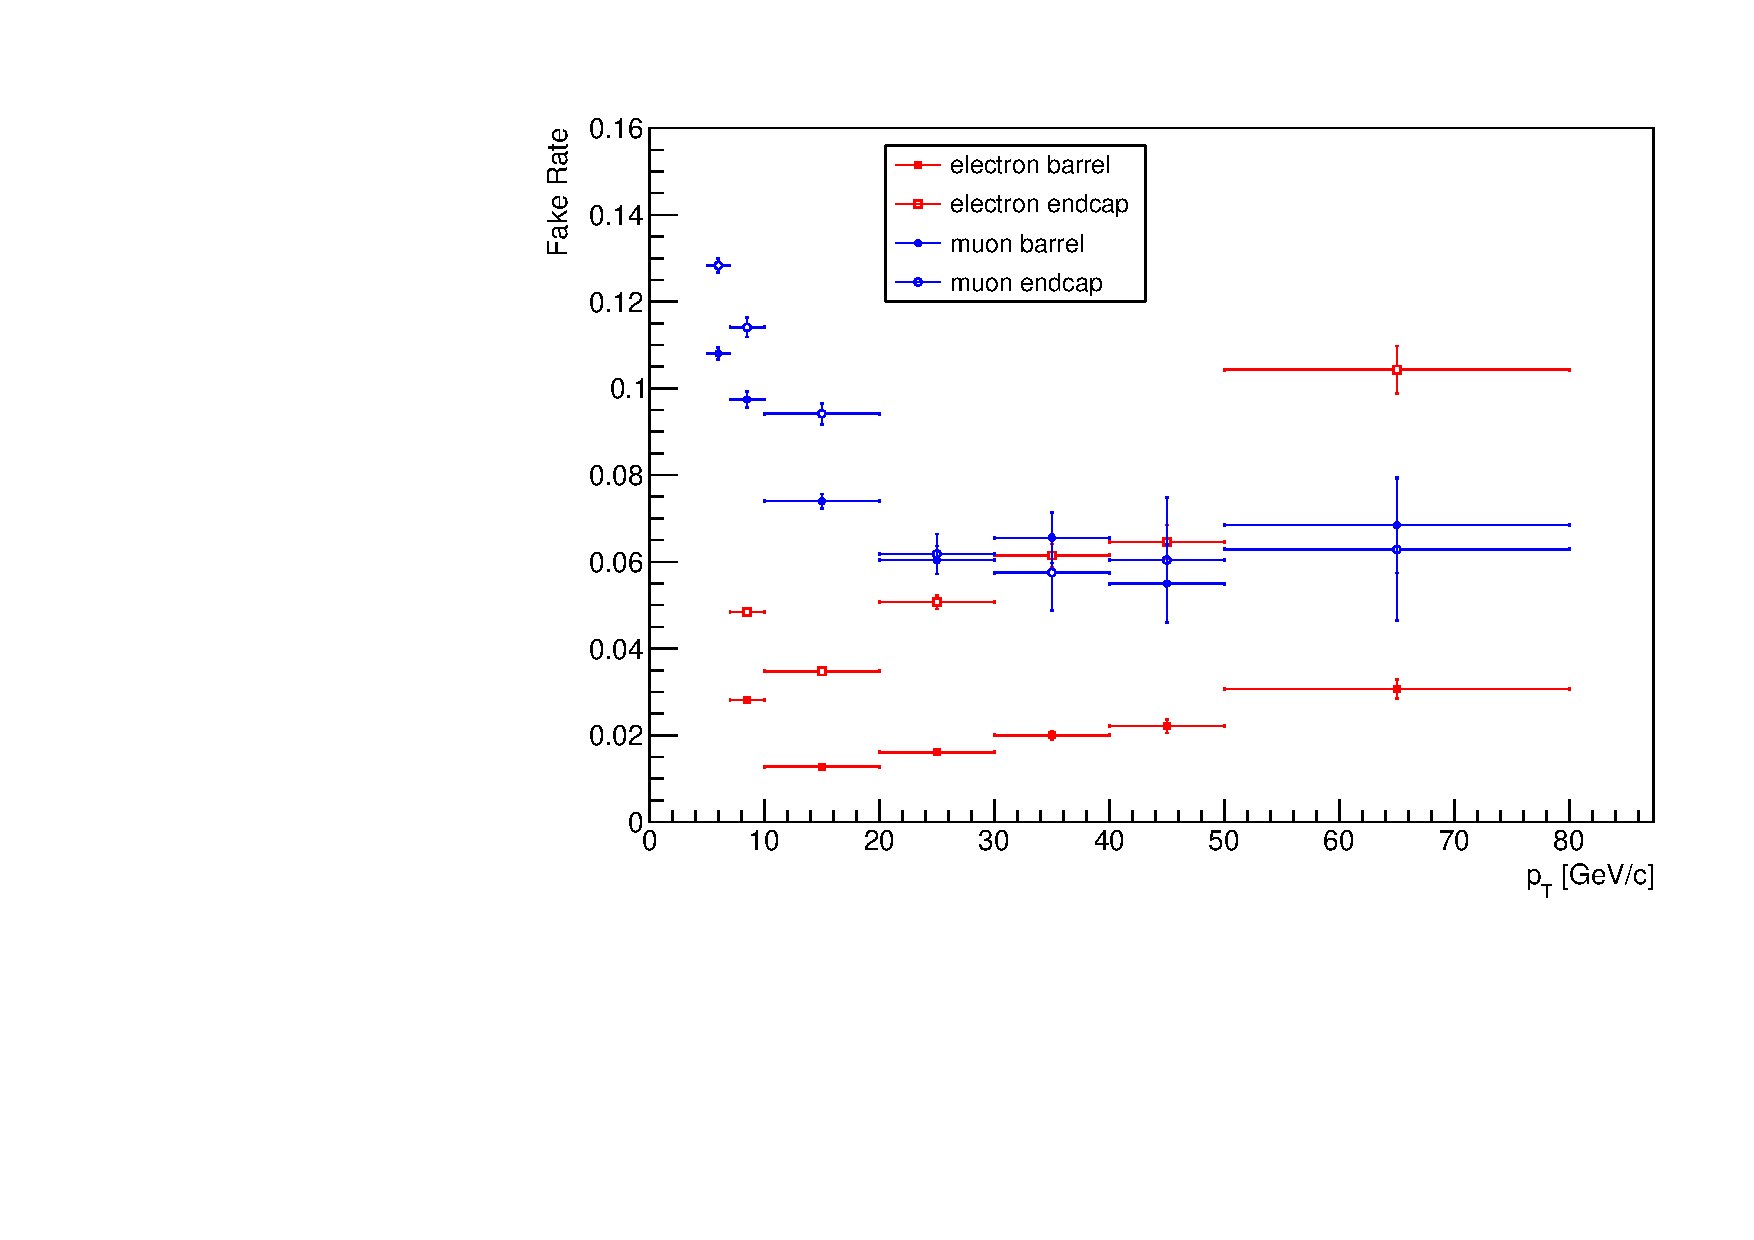
\includegraphics[width=.5\textwidth]{leptonFakeRate_2016.pdf}}%
  \subfigure [2017] {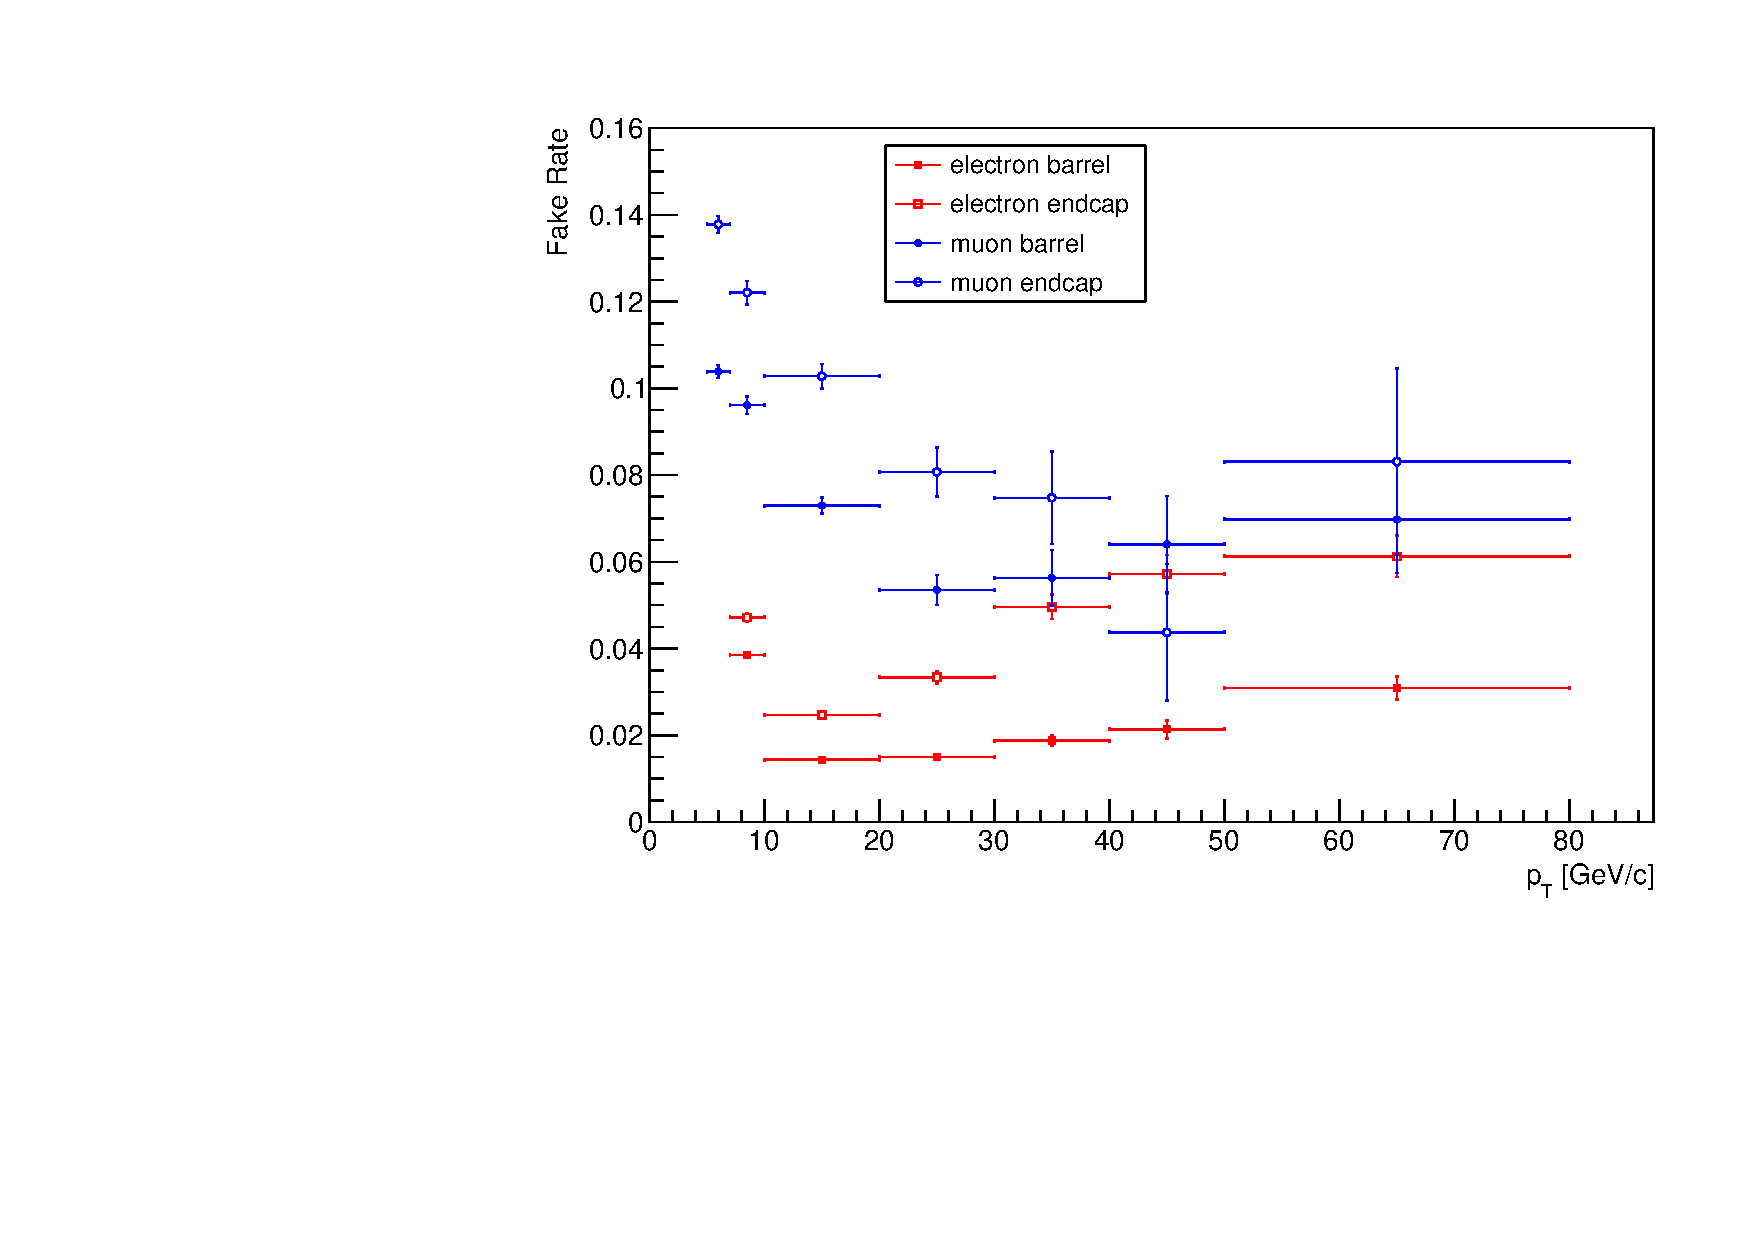
\includegraphics[width=.5\textwidth]{leptonFakeRate_2017.pdf}}\\
  \subfigure [2018] {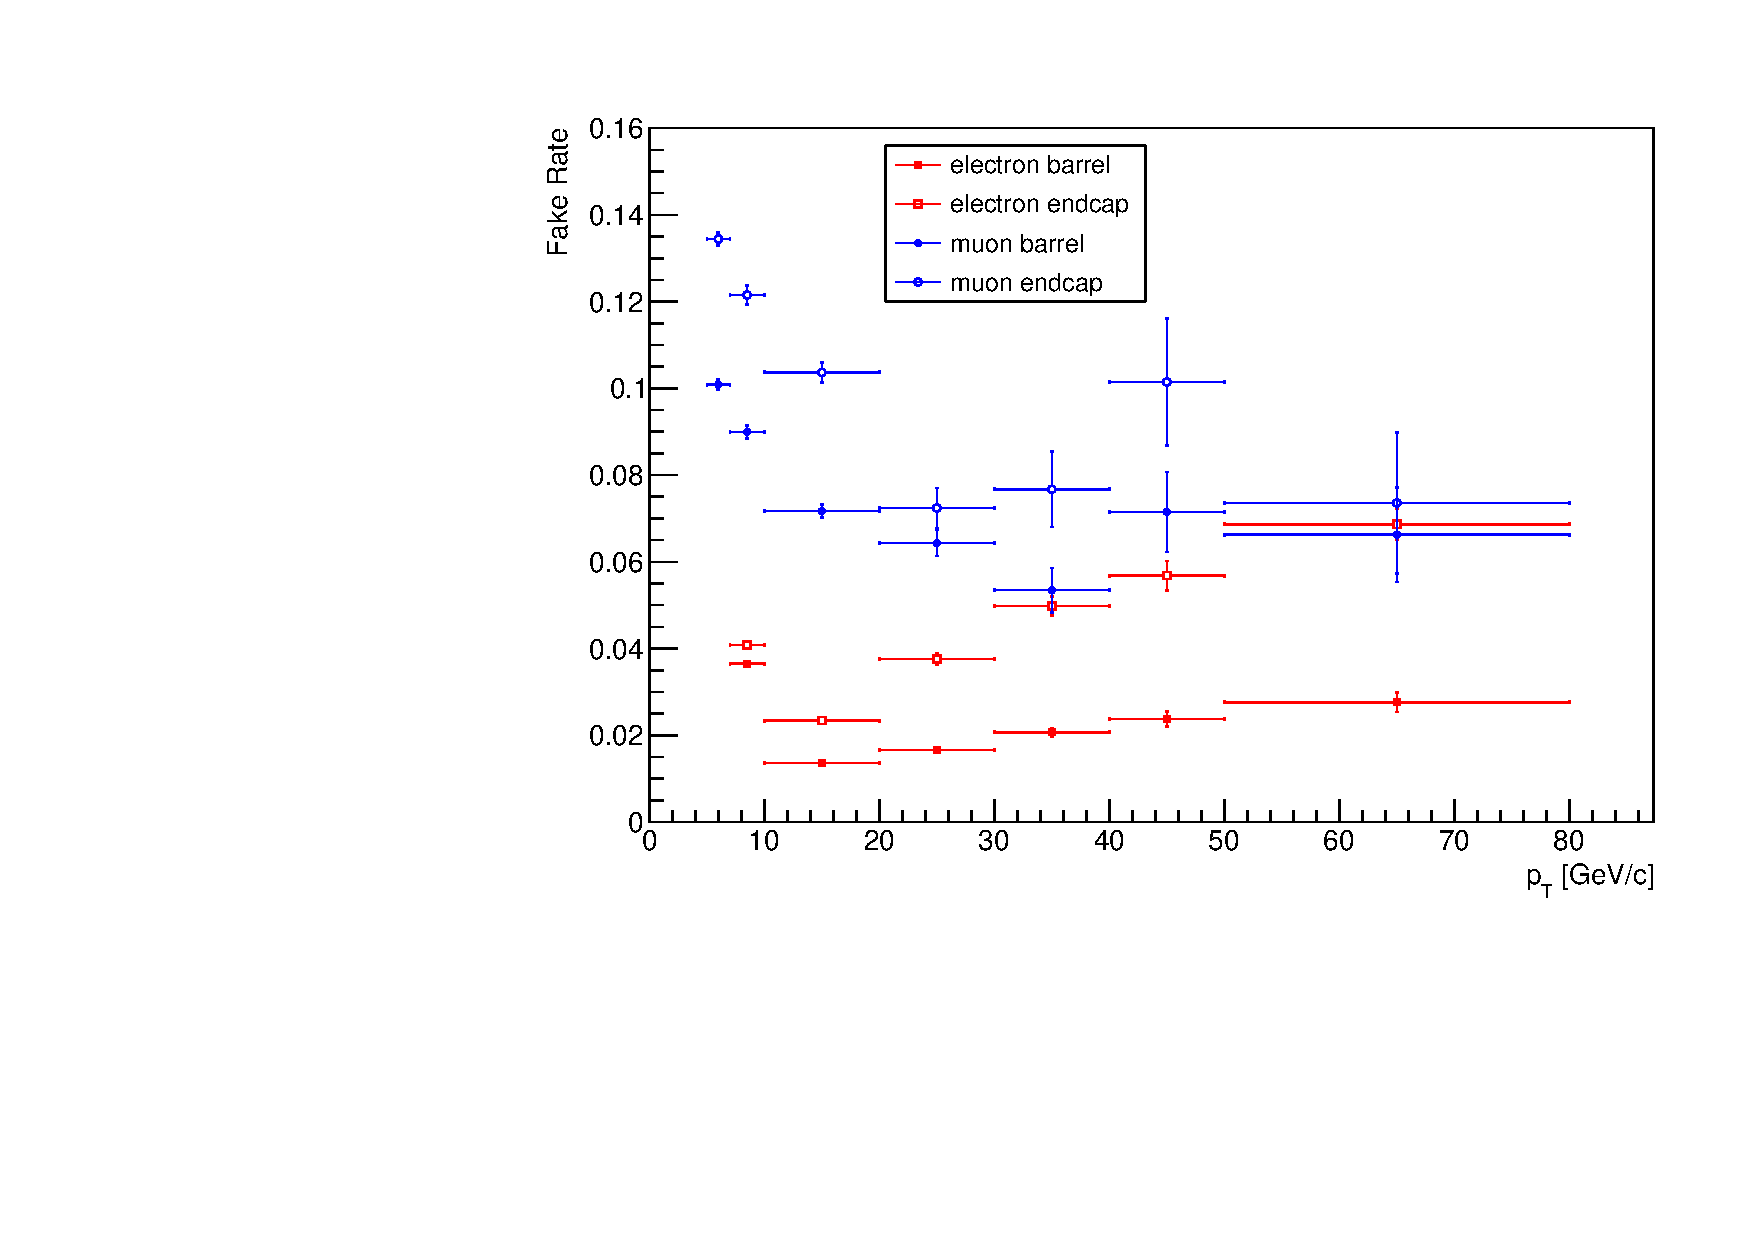
\includegraphics[width=.5\textwidth]{leptonFakeRate_2018.pdf}}
  \caption{Lepton fake rates measured in the $\PZ+L$ control region, for each year of data-taking.}
  \label{fig:leptonFR}
\end{figure}

The uncertainty on the fake lepton background estimation arises from the difference in composition of the
background processes in the region where the fake rate is measured and where it is applied.
This uncertainty was measured by several analyses \todo{cite} and found to be \todo{how much?}.


\paragraph{Lepton fake rate application\\}
Once the fake rates are estimated they are used to reweight the events
in dedicated control regions (alternatively called application regions).

\subsubsection{Four leptons channel}
% Description of the leptonic control regions with 4 leptons:
%  - the backgrounds
%  - data/MC plots
%  - table with fake_lepton background yield foreach year

\label{sec:lepCR4l}
Two control regions are defined for the 4\Pl channel with the same requirements as the signal region
except for the selection of one or more leptons, so as to be enriched in \nonprompt and misidentified leptons.
This method was used by several analyses targeting a final state with four leptons from $\PZ\PZ$ decay~\cite{CMS-SMP-16-001, CMS-SMP-17-006, CMS-SMP-20-001, CMS-PAS-SMP-22-001},
and is described in detail in Reference~\cite{CMS-HIG-13-002} as the ``Method using opposite-sign (OS) leptons''.

\paragraph{CR3P1F\\}
In the first region, named CR3P1F, one of the leptons of the $\PZ_2$ must fail (1F) the tight selection,
while the other three (both leptons from $\PZ_1$ and the other lepton from $\PZ_2$) must pass the tight identification and isolation criteria (3P).
It is expected to be populated by $\PW\PZ$, with contributions from Drell-Yan and $\PZ\PGg$,
along with a fraction of events from $(\PQq\PAQq/\Pg\Pg) \to \PZ\PZ$ where one of the prompt leptons fails the selection
or falls outside the acceptance and a misidentified jet is reconstructed instead.
Distributions of a few interesting kinematic observables are shown in Figure~\ref{fig:CR3P1F_Run2}.

\begin{figure}
\subfigure [$m_{\PZ_1}$     ] {\includegraphics[width=.333333333\textwidth]{Figures/dataMC_noLFR/Run2/fullMC/CR3P1F/Z0_mass_pow.pdf}}%
\subfigure [$m_{\PZ_2}$     ] {\includegraphics[width=.333333333\textwidth]{Figures/dataMC_noLFR/Run2/fullMC/CR3P1F/Z1_mass_pow.pdf}}%
\subfigure [$m_{\PZ\PZ\PGg}$] {\includegraphics[width=.333333333\textwidth]{Figures/dataMC_noLFR/Run2/fullMC/CR3P1F/ZZG_mass_loosePh_pow.pdf}}
\caption{Invariant mass of the $\PZ_1$, $\PZ_2$ (left and centre) without any request on the presence of a photon
  and mass of the $\PZ\PZ\PGg$ system (right) when there is a photon passing the cut-based ID selection,
  in the leptonic control region CR3P1F where one of the leptons from $\PZ_2$ fails the tight selection.}
\label{fig:CR3P1F_Run2}
\end{figure}

\paragraph{CR2P2F\\}
In the second region, named CR2P2F, both leptons from the $\PZ_2$ fail the tight selection (2F), while the leptons of the $\PZ_1$ pass the tight criteria (2P).
This region is populated primarily by Drell-Yan events, with contributions from $\PZ\PGg$ and $\PQt\PAQt+X$.
Some representative distributions for this region are shown in Figure~\ref{fig:CR2P2F_Run2}

\begin{figure}
\subfigure [$m_{\PZ_1}$     ] {\includegraphics[width=.333333333\textwidth]{Figures/dataMC_noLFR/Run2/fullMC/CR2P2F/Z0_mass_pow.pdf}}%
\subfigure [$m_{\PZ_2}$     ] {\includegraphics[width=.333333333\textwidth]{Figures/dataMC_noLFR/Run2/fullMC/CR2P2F/Z1_mass_pow.pdf}}%
\subfigure [$m_{\PZ\PZ\PGg}$] {\includegraphics[width=.333333333\textwidth]{Figures/dataMC_noLFR/Run2/fullMC/CR2P2F/ZZG_mass_loosePh_pow.pdf}}
\caption{Invariant mass of the $\PZ_1$, $\PZ_2$ (left and centre) without any request on the presence of a photon
  and mass of the $\PZ\PZ\PGg$ system when there is a photon passing the cut-based ID selection,
  in the leptonic control region CR2P2F where both leptons from $\PZ_2$ fail the tight selection.}
\label{fig:CR2P2F_Run2}
\end{figure}

\paragraph{Contribution to signal region\\}
The expected reducible background in the signal region is given by the sum of two terms:
\begin{itemize}
  \item A 3P1F component, from events with one fake lepton, estimated from the CR3P1F region.
  \item A 2P2F component, from events with two fake leptons, estimated from the CR2P2F region.
\end{itemize}

The 3P1F and 2P2F components are given by the number of events in the respective regions, weighted by factors dependent on the fake rates:
\begin{subequations}
  \begin{align}
    \label{eq:lepFR_3P1Fto4P}
    N^{\text{from 3P1F}}_{\text{SR}} &= \sum_{i \ins \text{3P1F}} \frac{f_a^i}{1-f_a^i}, \quad \text{where } a = 3 \text{ or } 4
    \\
    \label{eq:lepFR_2P2Fto4P}
    N^{\text{from 2P2F}}_{\text{SR}} &= \sum_{i \ins \text{2P2F}} \frac{f_3^i}{1-f_3^i} \frac{f_4^i}{1-f_4^i}
  \end{align}
\end{subequations}
where $f_3^i$ and $f_4^i$ correspond to the fake rates of the two loose leptons in the $i$-th event.

However, the CR3P1F region itself has a contribution from fake lepton background events from the CR2P2F region.
These are events with two genuine leptons and two fakes, where only one of the fakes passes the tight selection, thus winding up in the CR3P1F region.
The expected number of background events in the CR3P1F region, $N^{\text{from 2P2F}}_{\text{3P1F}}$,
can be computed from the number of events observed in the CR2P2F control region, $N^{\text{bkg}}_{\text{2P2F}}$,
by weighting each event in the region with a factor dependent from the fake rates:
\begin{equation}
  \label{eq:lepFR_N3P1F}
  N^{\text{from 2P2F}}_{\text{3P1F}} = \sum_{i \ins \text{2P2F}} \left( \frac{f_3^i}{1-f_3^i} + \frac{f_4^i}{1-f_4^j} \right)
\end{equation}

Summing all the contributions, one obtains for the signal region:
\begin{equation}
  \begin{split}
    \label{eq:lepFR_4P}
    N^{\text{bkg}}_{\text{SR}} &= \sum_{i \ins \text{3P1F}} \frac{f_a^i}{1-f_a^i} \left( 1 - N^{\text{from 2P2F}}_{\text{3P1F}} \right)
                               + \sum_{i \ins \text{2P2F}} \left( \frac{f_3^i}{1-f_3^i} \frac{f_4^i}{1-f_4^i} \right)
    \\
                 &= \sum_{i \ins \text{3P1F}} \frac{f_a^i}{1-f_a^i} - \sum_{i \ins \text{2P2F}} \left( \frac{f_3^i}{1-f_3^i} \frac{f_4^i}{1-f_4^i} \right)
  \end{split}
\end{equation}

More details on the derivation of Equation~\ref{eq:lepFR_4P} can be found in Appendix~\ref{sec:leptonFR_details}.


\subsubsection{Three leptons channel}
\label{sec:lepCR3l}
\note{At the moment, the data-driven fake estimate does NOT work in SR3P. Maybe we shouldn't discuss it if we don't use it.}

\note{SMP-16-002~\cite{SMP-16-002} (2015 data) uses a dijet region to measure the fake rate:
\textit{``The misidentification probability is measured from a sample of
dijet events enriched in nonprompt leptons. The sample is selected
with one jet passing the relaxed lepton identification requirements
matched to a single lepton trigger, defined as the probe lepton.''}}

\note{SMP-20-014~\cite{SMP-20-014} (full Run2) uses a L+j region:
\textit{``This CR is defined by requiring a single lepton with pT greater than 10 GeV, and at least
a reconstructed jet that is well separated from the lepton at $\DR(\PGg, j) > 0.7$. Contributions from
EWK processes are subtracted to obtain a pure nonprompt measurement region.''}}

Seven leptonic control regions are defined for the three lepton channel, following the strategy used in Reference~\cite{SMP-20-014},
using the same selections as the signal region except for the lepton identification.
The leptons are ordered: $\Pl^\PZ_1$, $\Pl^\PZ_2$ and $\Pl^\PW$
and the regions are defined based on which lepton fails the tight selection.
Unlike the four lepton channel the order is important,
so for example an event where only the leading lepton from the \PZ fails will be in a different control region
from an event where only the subleading lepton does not pass the tight selection.

This classification produces three regions where only one lepton fails the selection, three where two leptons fail and one where all three leptons are \nonprompt.
The agreement between the simulation and the data decreases accordingly, given the instrumental nature of this background, which makes it difficult to model.

\begin{figure}
  \subfigure [$\Pl^\PW$ fails  ] {\includegraphics[width=.333333333\textwidth]{Figures/dataMC_noLFR/Run2/fullMC/CR110/lll_mass_pow.pdf}}%
  \subfigure [$\Pl^\PZ_1$ fails] {\includegraphics[width=.333333333\textwidth]{Figures/dataMC_noLFR/Run2/fullMC/CR011/lll_mass_pow.pdf}}%
  \subfigure [$\Pl^\PZ_2$ fails] {\includegraphics[width=.333333333\textwidth]{Figures/dataMC_noLFR/Run2/fullMC/CR101/lll_mass_pow.pdf}}
  \caption{Invariant mass of the three charged leptons in the three lepton control regions for the 3L channel where only one lepton fails the selection.}
  \label{fig:CR3L_1_Run2}
\end{figure}

\begin{figure}
  \subfigure [$\Pl^\PZ_1$ and $\Pl^\PZ_2$ fail] {\includegraphics[width=.333333333\textwidth]{Figures/dataMC_noLFR/Run2/fullMC/CR001/lll_mass_pow.pdf}}%
  \subfigure [$\Pl^\PZ_1$ and $\Pl^\PW$ fail  ] {\includegraphics[width=.333333333\textwidth]{Figures/dataMC_noLFR/Run2/fullMC/CR010/lll_mass_pow.pdf}}%
  \subfigure [$\Pl^\PZ_2$ and $\Pl^\PW$ fail  ] {\includegraphics[width=.333333333\textwidth]{Figures/dataMC_noLFR/Run2/fullMC/CR100/lll_mass_pow.pdf}}
  \caption{Invariant mass of the three charged leptons in the three lepton control regions for the 3L channel where two leptons fail the selection.}
  \label{fig:CR3L_2_Run2}
\end{figure}


\subsubsection{Two leptons channel}
\label{sec:lepCR2l}
The preliminary strategy for the two lepton channel is to use a data-driven estimate of fake photons
which, as described in Section~\ref{sec:backgrounds_in_SR}, does not need the data-driven estimate of \nonprompt leptons.

A potential strategy for the estimation of the fake lepton contribution in the signal region of this channel was formulated,
emloying employing procedures similar to those applied in the other two.
The fake rate measured in the $\PZ+\rm{L}$ region is applied to reweight events in two control regions: CR1P1F and CR0P2F.
These regions contain a massive amount of events.
The region CR1P1F in particular has a significant contribution from $\PW+\text{jets}$ events,
while the CR0P2F is dominated by QCD-induced jet production.
The event weights applied to derive the contribution to the signal region are the same used in the four lepton channel,
which account for the contamination of the region with one lepton failing the tight selection from events with two fake leptons.


